\documentclass[]{report}
\usepackage{graphicx}
\usepackage{apacite}
\usepackage{times}
\usepackage{amssymb}
\usepackage{amsmath}
\usepackage{amsthm}
\usepackage{wrapfig}

%% Margin control
\textwidth 7.0in
\oddsidemargin -0.25in
\textheight 9.5in
\topmargin -0.75in

\begin{document}
\section*{Genthor}
\subsection*{Goal}
\setlength{\intextsep}{-40pt}
\begin{wrapfigure}[10]{r}{0.3\textwidth}
\vspace{-70pt}
%\begin{figure}[ht]
\centering
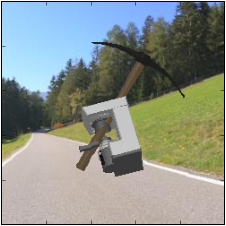
\includegraphics[width=0.3\textwidth]{example.png}
\caption{Example image}
%\label{fig:gen-model}
\end{wrapfigure}
%\end{figure}
\setlength{\intextsep}{40pt}

Developing a system for visual inference about naturalistic scenes
with multiple objects arranged in depth.

\subsection*{Definitions}
We focus on simple 3D scenes, $s \in \mathcal{S}$, that consist of a
background ($o_0$) that has a unique ID, $b$, and two spherical
rotation coordinates, $(r_{x,0}, r_{y,0})$, plus a set of foreground
objects ($n < 6$, for now) $(o_1,\dots,o_n)$, each of which belongs to
one category, $c_i$, has 3 position coordinates,
$(p_{x,i},p_{y,i},p_{z,i})$, 3 scale coordinates,
$(w_{x,i},w_{y,i},w_{z,i})$, and 3 rotation coordinates,
$(r_{x,i},r_{y,i},r_{z,i})$.  The scene is unobserved, but it
generates images, $d \in \mathcal{D}$, through a rendering function,
$\mathrm{R}(\cdot)$, plus some noise, $\omega$.
\begin{align*}
  s &= (n,o_0,o_1,\dots,o_n)\\
  o_0 &= (b, r_{x,0}, r_{y,0})\\
  o_i &= (c_i, x_i,y_i,z_i, w_{x,i},w_{y,i},w_{z,i}, r_{x,i},r_{y,i},r_{z,i});\ i > 0\\
  d &= \mathrm{R}(s) + \omega
\end{align*}
We assume all values are discrete.

\subsection*{Generative model}
The generative model specifies our assumptions about how scenes
generate images using prior and conditional probability distributions,
$\Pr(S=s)$ and $\Pr(D=d | S=s)$, using a joint probability distribution: 
\[
\Pr(D=d,S=s) = \Pr(D=d | S=s)\Pr(S=s)
\]
We abbreviate $\Pr(X=x)$ as $\Pr(X)$.  We can draw $(S,D)$ samples and
evaluate their probabilities. A simple example is:
\begin{align*}
  \Pr(S) &= \mathrm{Unif}(S)\\
  \Pr(D | S) &= \mathrm{Normal}(D; \mathrm{R}(S), \sigma_d)
\end{align*}

\subsection*{Inference}
Visual scene inference is defined as computing the Bayesian posterior
distribution,
\[
\Pr(S | D) = \frac{\Pr(D | S)\Pr(S)}{\sum_S \Pr(D | S)\Pr(S)}
\]
Since $\mathrm{R}^{-1}(D)$ is one-to-many and undefined, analytical
methods are hard to develop.  Monte Carlo sampling can be used to draw
posterior scene samples, $\{\tilde{S}_0,\dots,\tilde{S}_N\}$, which
support expectations, modes, density estimates, etc. Rejection or
importance sampling using proposals from the prior is inefficient
because the latent space is large. Instead, we use proposals drawn
from a feedforward discriminative model (Thor) to target high
probability of the latent space.

We approximate the unormalized posterior, $\Pr(S | D) \approx \pi(S;
D)$.

\subsubsection*{Thor (Dan -- fill in / correct)}
Thor is a system for feedforward visual recognition, based on
convolutional neural networks, that uses a sequences of nonlinear
filtering operations to compute a feature vector that supports linear
classification of objects. The input is a multichannel 2D image. Each
filtering step is composed of 5 sub-steps: 1. Linear filtering through
random projections, 2. Activation nonlinearity (sigmoid), 3. Pooling,
4. Normalization (optional), 5. Rescaling (subsampling). The output is
a feature vector(/tensor?), $F \in \mathcal{F}$, that is input to a
linear SVM. The training uses a sort of backpropagation (Is this
true?? how does it learn?).

Abstractly, Thor defines a map, $\mathrm{T}$, from images,
$\mathcal{D}$ to a set of feature vectors, $\mathcal{F}$, and a map,
$\tau$, from $\mathcal{F}$ to a subset of the latent scene state,
$\mathcal{U}_j \subseteq \mathcal{S}$:
\begin{align*}
  \mathrm{T}(\cdot, \theta) &: \mathcal{D} \rightarrow \mathcal{F}\\
  \tau(\cdot, \lambda) &: \mathcal{F} \rightarrow \mathcal{U}_j
\end{align*}
where $\theta$ and $\lambda$ are parameters.

The parameters, $\theta$ and $\lambda$, are learned through training
on a set of virtual examples, $\{(D^{(k)}, U^{(k)});\ k=1, \dots,
K\}$, by minimizing the distances, $f(\cdot,\cdot)$, between scene
labels and predictions:
\begin{align*}
  \underset{\theta, \lambda}{\operatorname{argmin}} \sum_{k=1, \dots, K}
  f(U^{(k)}, \tau(\mathrm{T}(D^{(k)}, \theta), \lambda)
\end{align*}

Thor's $\tau$ can instead map to a real-valued measure, $\mu \in
\mathcal{M}$, of the credibility, $e \in \mathcal{E}$, over elements
in $\mathcal{U}_j$ given $\mathcal{F}$:
\begin{align*}
  \tau(\cdot, \lambda) &: \mathcal{F} \rightarrow \mathcal{M}\\
  \mu(\cdot) &: \mathcal{U}_j \rightarrow e
\end{align*}
By normalizing, $\mu$ can approximate the posterior over $U$:
\begin{align*}
  \Pr(U|D) \approx \frac{\mu(U)}{\sum_U \mu(U)}
\end{align*}
When $\mathcal{U}_j$ is a strict subset of $\mathcal{S}$, then for
$\mathcal{B} = \mathcal{U}_j \setminus \mathcal{S}$, $\Pr(U|D)$ is the
posterior with $B$ marginalized out,
\begin{align*}
  \Pr(U|D) = \sum_B \Pr(S|D) \text{,}
\end{align*}
and when $\mathcal{U}_j$ contains only one type of element (e.g.,
$p_{x,i}$) then, $\Pr(U|D)$ is the posterior marginal distribution
over that element.


\subsubsection*{Rejection/importance sampling}
Thor's predicted posterior marginals can be used as a proposal
distribution for a rejection or importance sampling
algorithm. Specifically, the sampler's proposal distribution is,
\begin{align*}
\mathrm{Q}(S) = \mathrm{Q}(U) \mathrm{Unif}(B)\\
\mathrm{Q}(U) = \mathrm{Multinomial}(\frac{\mu(U)}{\sum_U \mu(U)}, n)
\end{align*}
where $n$ is a set number of objects (which could, itself, be predicted by Thor).

For rejection sampling, the samples' acceptance probability is,
\begin{align*}
  a_j = \frac{\Pr(S_j | D)}{C \mathrm{Q}(S_j)}
\end{align*}
where $C$ is the rejection factor.

For importance sampling, the samples' (unnormalized) importances
weights are,
\[
w_j = \frac{\Pr(S_j | D)}{\mathrm{Q}(S_j)}
\]

\subsubsection*{Likelihood based on features}
In reality, 
\[
\Pr(D | S) \approx 
\begin{cases}
  1 , & \text{if } D = \mathrm{R}(S) \\
  0 , & \text{otherwise}
\end{cases}
\]
But in general, for most $D$ the set $\{S;\ D = \mathrm{R}(S)\}$ is
relatively small, i.e.,
\[
\frac{|\{S;\ D = \mathrm{R}(S)\}|}{|\{S\}|} = \epsilon
\]
where $\epsilon$ is exponentially small in $|S|$. Thus, $\Pr(D | S)$
does not easily support Monte Carlo sampling.

We seek an approximation to $\Pr(D|S)$ that will make inference
easier.  Our goal is to find distance kernels, $\delta(D_0, D_1)$ and
$\delta'(S_0, S_1)$, where $D_k = \mathrm{S_k}$,


induce a qualitative isomorphism between

Approximations that put a noise term on the pixels might help
soften the posterior, but it does not 

Target: small covariance
$\mathrm{E}[\delta(D_0, D_1) \delta'(S_0, S_1)]$.  Is this a good way to define
the problem -- Spearman correlation? Pearson?  Mutual information?

Our solution is to use an alternative rendering function,
\begin{align*}
  \mathrm{R}^* = \mathrm{R} \circ \mathrm{T} : \mathcal{S} \rightarrow \mathcal{D} \rightarrow \mathcal{F}\\
  \Pr(F | S) = \mathcal{N}(F;S, \sigma_F)
\end{align*}

Spearman rank correlation

ABC?


\end{document}